\chapter{Prosessdokumentasjon}
\marginpar{
Test for sitering av kilder.\cite{forelesning:tulpesh}\cite{book:utforming}\cite{book:desintsystems}
}
\lettrine[lines=2]{I}{} følgende kappitel beskriver vi hvordan hele utviklinsprosessen for protitypene har foregått. Hensikten er at man skal illustrere hele prosessen fra idé, mockup til hi-hi prototype klar for brukertesting. Kapitlet består av mange for å på enklest muli måte ilustrere prosessen. for eventuell beskrivelse av funksjonalitet av de inngående moduler som er synlige på bildene henvises til appediks \ref{app:funksjonalitet}.




\section{Første utkast}
\marginpar{Viktige prinsipper:
feedback, constraints (bruker får ikke gjøre feil), affordances
}
\marginpar{Støtteord:
Usability (brukbarhet): konsistens, brukerkontroll, passende presentasjon.
}
Etter at idéen om hva vi skal jobbe med var klar og diskutert tok det ikke lang tid før vi ble enige om hvordan vi skal sette sammen vårt forslag til en helhet. Hele gruppen var tydelig på at vi ønsker i stor gra å benytte oss av en løsning som baserer seg tydelig på gestalt prinsipper.
Det som var spesielt viktig var at man deler opp de forskjellige moduler i flere undermoduler slik at de bilder en visuell og logisk helhet. 
Forslaget var ganske klart opplegg der alle viktige moduler blir satt asmmen i en overordnet gruppe som disse tilhører. I det første utkastet bestod disse av:
\begin{center}
Editorer | Meldinger | Resurser | System | Servers
\end{center}
Dessa skulle plaseres på en velkomstside som innholdr også annen viktig informasjon for brukeren. Man skal bli presnetert med sin brukerikone i øvre høyre hjørn pg en hurtigtilgang til systeminstillinger. Under skal det også eventuelt presenteres noen <<widgets>> som viser systemstatus, påloggede bruker, andel brukt ram-minne, tilgjengelig lagringsplass og kjørende prosesser. Alt dette blir pakket ned til en dynamisk nettside og vil være tilgjengelig via en webbrowser. Muligheten å kontrollere systemet via en webbrowser gjør det mulig til å styre oppsettet av systemet fra hvilken manskin man enn ønsker og eventuelle tilpassninger kan også gjøres slik at konfigurasjonen kan også foregår fra nettbrett eller telefon.

Det som er viktigst for oss her er at man samler opp komponentene på en spesifikk måte som gjør brukeropplevelsen så enkel som mulig. Vi synes ikke at brukeren skal behøve <<tenke>> over hvordan systemet skal brukes. Det skal være mulig for hvilken som helst person med noe data vane å begynne benytte systemet kun etter en rask overblikk av de grafiske komponentene på fremsiden.
Presentasjonen skal være passende for de oppgave som systemet er tenkt at det skal gjøre. Det er derfor ingen anledning å overkomplisere noen av komponentene på grunn at f.eks. eliminere tom plass på siden. Den tomme plassen som er synlig i utkastet er tenkt at den skal brukes til å plassere menyer som skal åpnes. Vi ser på dette utkastet som at det ser inviterede ut til interaksjon ettersom det er få komponenter som er plasert i proksimitet til hverandre (mer om brukte gestalt prinsipper i avsnitt \ref{sec:lowfi}). Slik plassering gjør det ganske enkelt å finne ut hva som skal benyttes og hvorfor. Dette kan ses på som <<constraints>> der brukeren ikke kan gjøre mye annet enn de funksjoner som gjør det mulig til å benytte seg av for tilfeldet.\cite{nielsen2000designing}



\begin{figure}
%bruk \begin{figure}[ht] dersom figuren ikke skal flyte
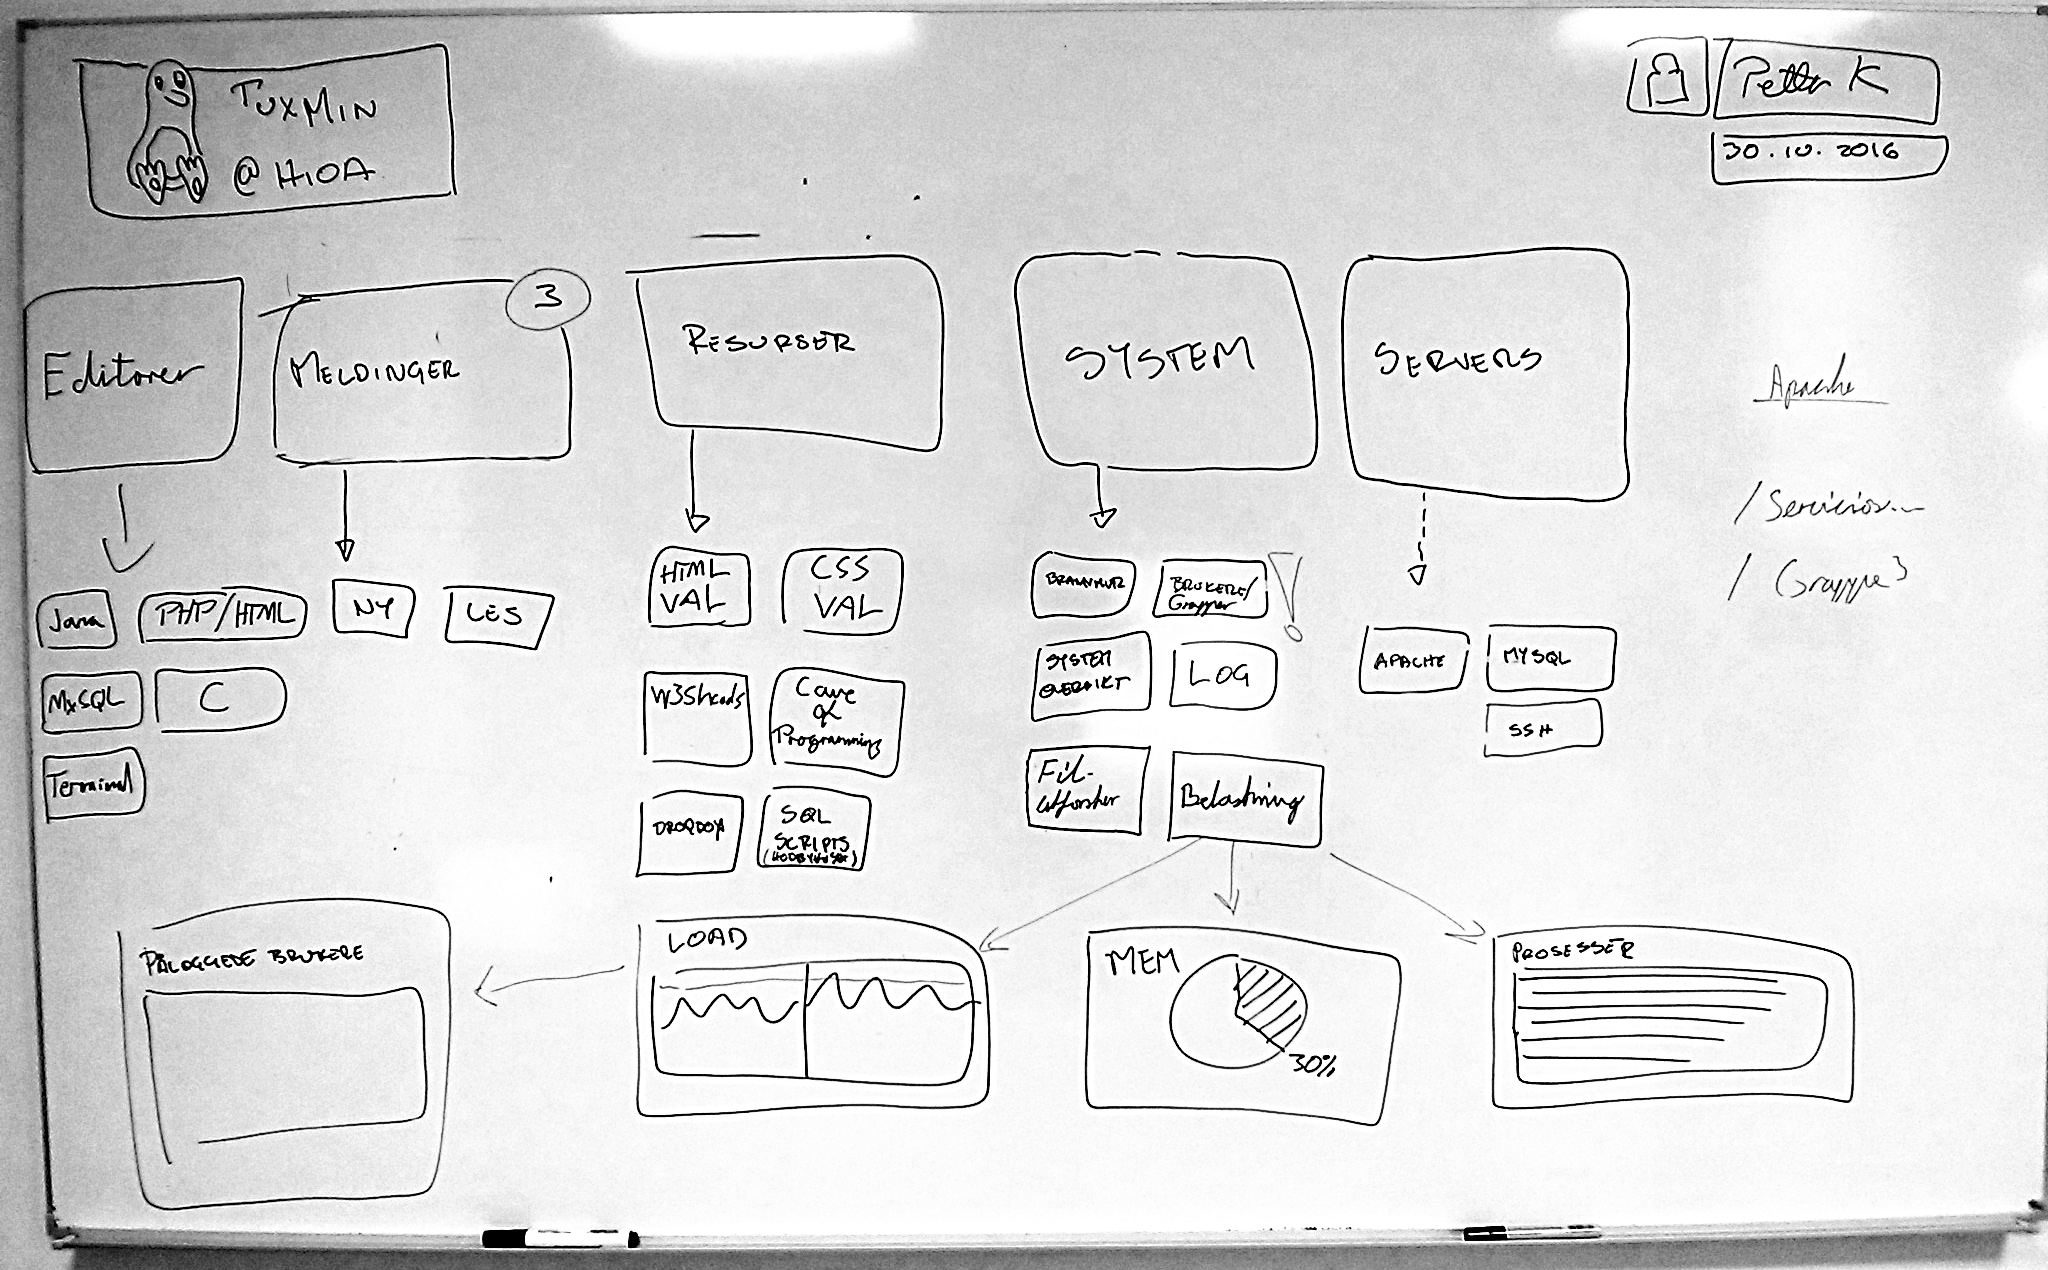
\includegraphics[width=\textwidth,height=\textheight,keepaspectratio]{./img/prosessdokumentasjon/foersteutkast/foerste.jpg}
\caption[Første utkast]{Første utkast over brukergrensesnittet.}
\label{fig:foersteutkast}
\end{figure}

\section{Low-fi prototype} \label{sec:lowfi}
Det er ganske vanlig at man til en low-fi prototype bruker papp eller papir fo rå visualisere hvordan man kan bruke en GUI. Vi valgte å benytte oss av \href{http://balsamiq.com/products/mockups/}{balsamiq mockups} hvilket gav oss mulighet å ikke bare visualisere hvordan brukergrensesnittet skulle se ut men også legge inn enkel funksjonalitet. Slik funksjonalitet bestod av at man fikk mulighet til å klikke seg videre til neste skjermbilda fra menyer. Dette gav en ganske grei opplevelse over hvordan det kommer til å føles da man bruker produktet.


Dersom vi tar en rask overblikk over framsiden i figur \ref{fig:lowfi_fremside} ser vi at hver enkel modul er gruppert etter gestalt prinsippen for proksimitet og elementer.\cite{forelesning:tulpesh}

Prototypen inkluderer eksempel over konfigurasjon over to forskjellige funksjoner.
Det er valig at i en prototype fokuserer man på en horisontell eller vertiklall implementasjon. Der i den horisontelle versjonen implementerer man få eller ingen funksjoner som går på dybden med insteden forsøker man å vise bredden av muligheter i et system eller grensesnitt. I den vertikale implementasjonen velger man insteden å begrense bredden på hva prototypen kan vise eller gjøre med insteden implementerer man en eller flere funksjoner på dybdeben.\cite{book:utforming}
På dette studium har vi valgt å avgrense disse til konfigurasjon av Apache webserver og oppsett av brukere og grupper. 

\begin{figure}
%bruk \begin{figure}[ht] dersom figuren ikke skal flyte
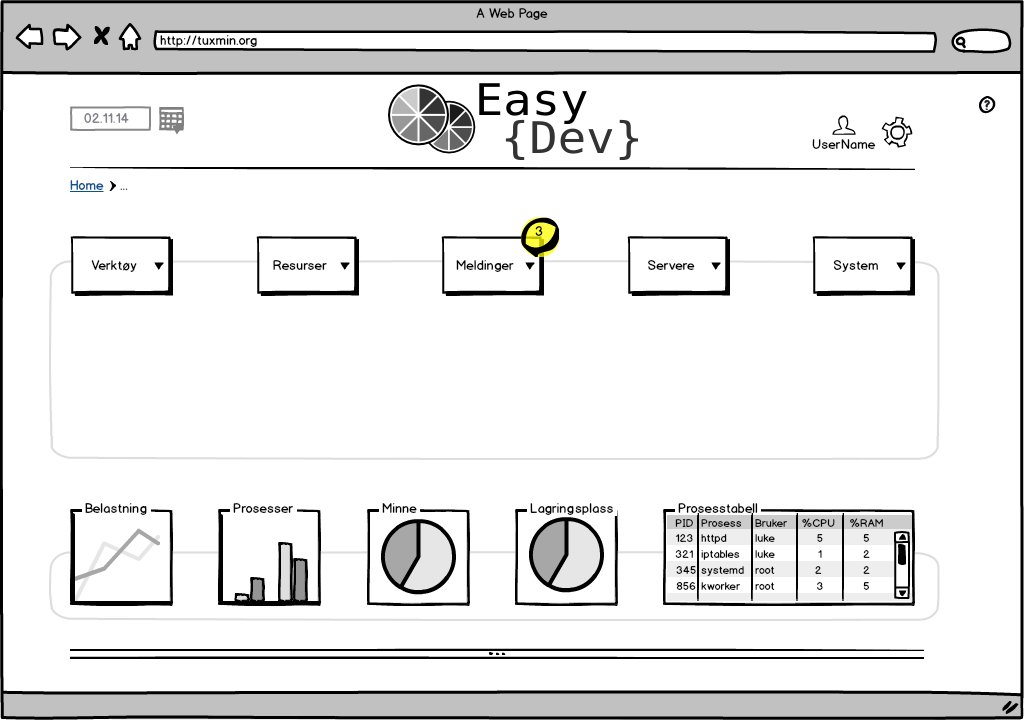
\includegraphics[width=\textwidth,height=\textheight,keepaspectratio]{./img/prosessdokumentasjon/lowfi/fremside.png}
\caption[Low-fi prototype]{Fremside for EasyDev i første low-fi prototype.}
\label{fig:lowfi_fremside}
\end{figure}


I etterfølgende seksjoner beskriver vi i detalj funksjonaliteeten til to moduler. Disse er grunnelgende moduler for systemet som har følgt med siden den ursprunglige idéen. Disse moduler er et godt eksempel på hvordan vi har tentk at produktet skal fungere. Derfør ønsker vi å beskrive de mer detaljert.

\subsection{Oppsett av apache webserver}
Her tentke vi gå nærmere på å vise hvordan det er tenkt at en submodul for konfigurasjon og oppsett av serverelement skal brukes. Alle trinn som beskrives er presentert i figur \ref{fig:lowfiapache}.

Vi utgår fra at dette er intuitiv å velge modul \texttt{Servere} dersom man ønsker å konfigurere en tjener. Modulen er tilgjengelig på fremsiden med en rullmeny som viser hvilke servere som vi har mulighet til å konfigurere, figur \ref{fig:apache1}. 
Apache webserver trenger å vite hvilke mapper som denne skal lese fra. Hvis man installerer apache på en Linux manskin kommer den som standard å lese fra mappe \texttt{/var/www} som har kun root tilgang. Vi vil ikke endre rettigheter for denne mappe ettersom de vi stride mot standarden for rettigheter i systemet og utgjøre en sikkerhetsrisiko.\cite{book:unixprog}
Det som vi ønsker å gjøre isteden er å definere om instllinger i Apache slik at serveren leser fra brukerens sin egen mappe. Dette er normalt en utfording ettersom det må gjøres i form av to til tre trinn:\footnote{Antall trinn her er ganske avhegig av hvilket Linux system som brukes}

\begin{itemize}
\item Endre konfigurasjon i apache.conf til å istedenfor eller i tillegg lese fra brukerens hjemmemappe. Det må opprettes en spesifikk mappe f.eks. \texttt{/home/bruker/html}. 
I noen tilfelder er det nødvendig å installere plugin \href{http://httpd.apache.org/docs/2.2/mod/mod_userdir.html}{\texttt{mod\_{}userdir}}. Dette vil gjøre det mulig å lese filene vis følgende adresse: \texttt{http://localhost/\~{}bruker/fil.html}

\item Endre rettigheter til den mappe i hjemmemappe som filene skal leses fra. Dette forutsetter at brukeren og Apache webserver er i samme brukeregruppe. Oftest må brukeren bli lagt til \texttt{www} eller \texttt{httpd} gruppe på systemet. Det er selvfølgelig mulig å åpne mappen helt slik at alle grupper i systemet vi ha tilgang til denne men slik tilnærming senker sikkerheten i stor grad i et flerbrukersystem. Dette er noen som lager en del vanskeligheter for nybegynnere og der man i starten faktisk velger å åpne mappen helt ettersom man oftest ikke har mulighet å teste dersom rettighetene er satt riktig hvis man har kun en bruker.

\item Systemer som benytter seg av SELinux (\href{http://en.wikipedia.org/wiki/Security-Enhanced_Linux}{Security Enhanced Linux}) må i tillegg legges til en policy der Apache skal få lov til å lese fra brukermapper. Dette er på grunn at SELinux er et oppsett av rettigheter som i tillegg overstyrer hvanlig skriv og leserettigheter i systemet på kernel nivå\footnote{Dette er ikke noe som vi skal beskrive i detalj og finnes her kun for å illustrere problemstilligen som bruekren kan bli utsatt for.}. 
\end{itemize}

Eksemplene over viser hvor vanskelig dt kan være å faktisk sette opp Apache webserver på sin egen maskin. Det er rett og slett mulig å skrive linkende lisete for hvert bilde i 
Dette er et primært ekesempel på område der EasyDev kommer inn med enkle løsninger. Apache modulen i EasyDev er tenkt at den skal opprette alle disse konfigurasjoner for å få en fungerende server.

Dersom vi se i figur \ref{fig:apache2} ser vi at undr oppsettet kan brukeren velge hvilke mapper som skal inkluderes i konfigurasjonen. Dette er mapper som webservern kommer til å ha mulighet å lese fra. 
I neste trinn (figur \ref{fig:apache3}) blir brukeren presentert i hvilke av de valgt mappende ønsker man å benytte for å aktivere <<directory browsing>>. Dette er en funksjon som gjør det mulig å se innholdet i mappe se tjenes av serveren direkte i nettleseren. Dette er normalt en funksjon som ikke brukes på en <<live>> server men er meget brukbart ved både utvikling og testing. 
Figur \ref{fig:apache4} viser hvilke typer av innstiksplugins som kan velges i tillegg til Apache installasjonen. Disse kan for eksempel være plugins som PHP eller MySQL eller andre. Hensikten er at man kan samla alle slike tillegg på en plass slika at brukeren kan også velge disse i et seinere tilfelde.
Siste eksempel (figur \ref{fig:apache5}) viser mulighet for konfigurasjon av noen av mer avanserte tillegsmoduler. Disse kan f.eks. være støtte for flere vituelle servere av Apache noe som gir bedre skalerbarhet ved utvikling av flere prosjekter parallellt. 
% med flagg p setter vi hele denne figuren på en egen side
\begin{figure}[!ht]
        \centering
        \begin{subfigure}[b]{0.48\textwidth}
                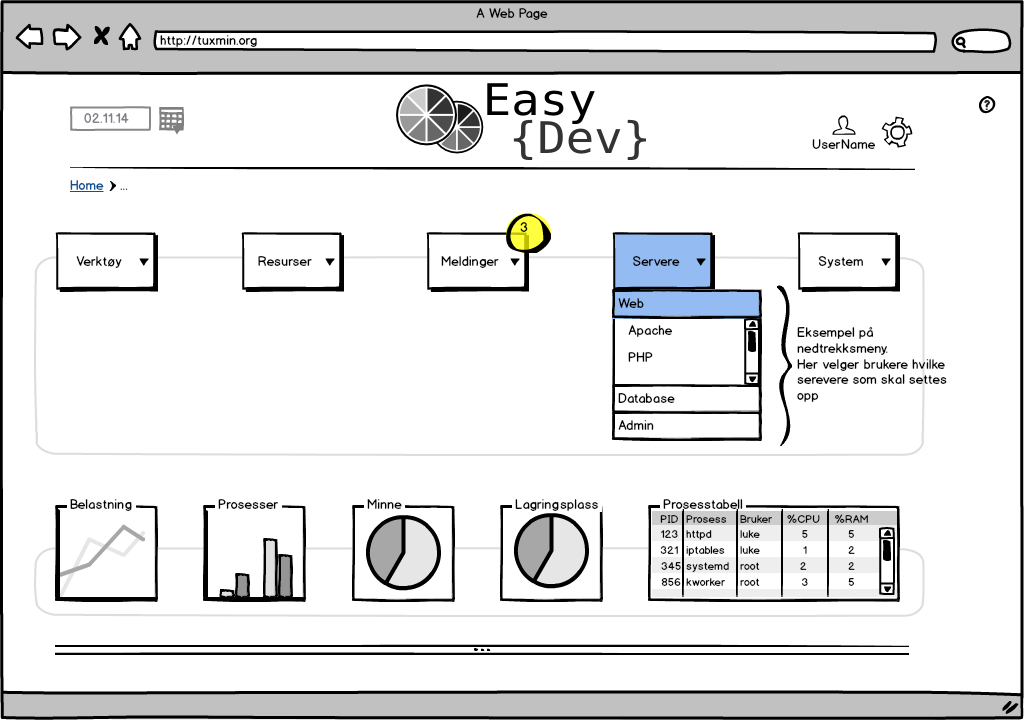
\includegraphics[width=\textwidth]
                {./img/prosessdokumentasjon/lowfi/apache1.png}
                \caption{Fremside -> Sett opp webserver}
                \label{fig:apache1}
        \end{subfigure}%
        ~ %add desired spacing between images, e. g. ~, \quad, \qquad, \hfill etc.
          %(or a blank line to force the subfigure onto a new line)
        \begin{subfigure}[b]{0.48\textwidth}
                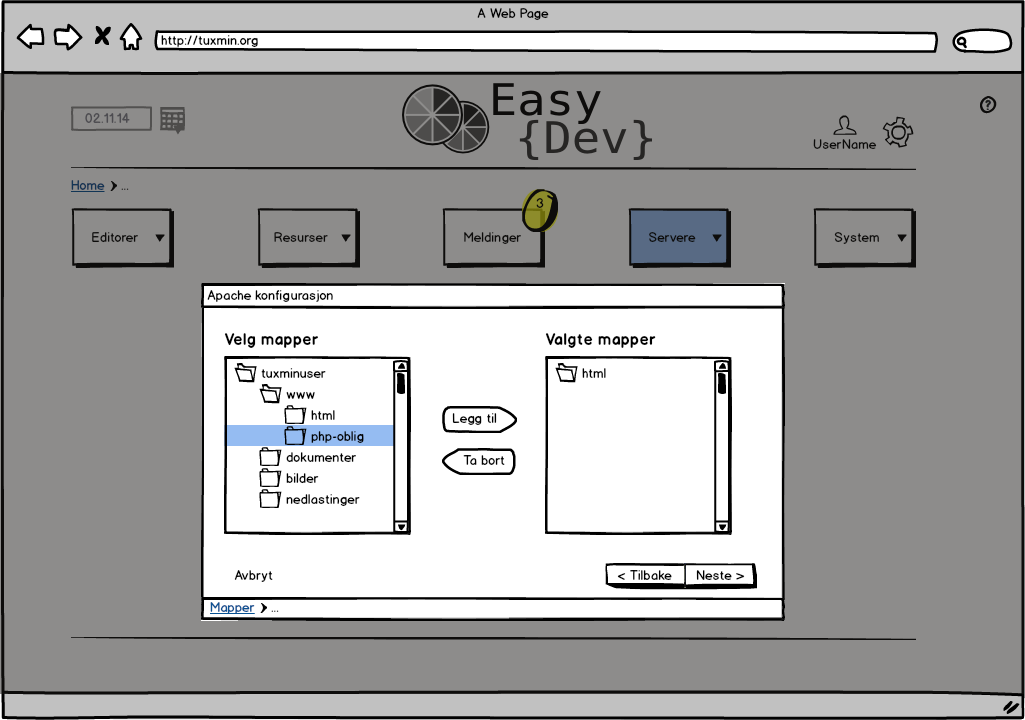
\includegraphics[width=\textwidth]
                {./img/prosessdokumentasjon/lowfi/apache2.png}
                \caption{Valg av mapper}
                \label{fig:apache2}
        \end{subfigure}
       
        \vspace{0.6cm}
        \begin{subfigure}[b]{0.48\textwidth}
                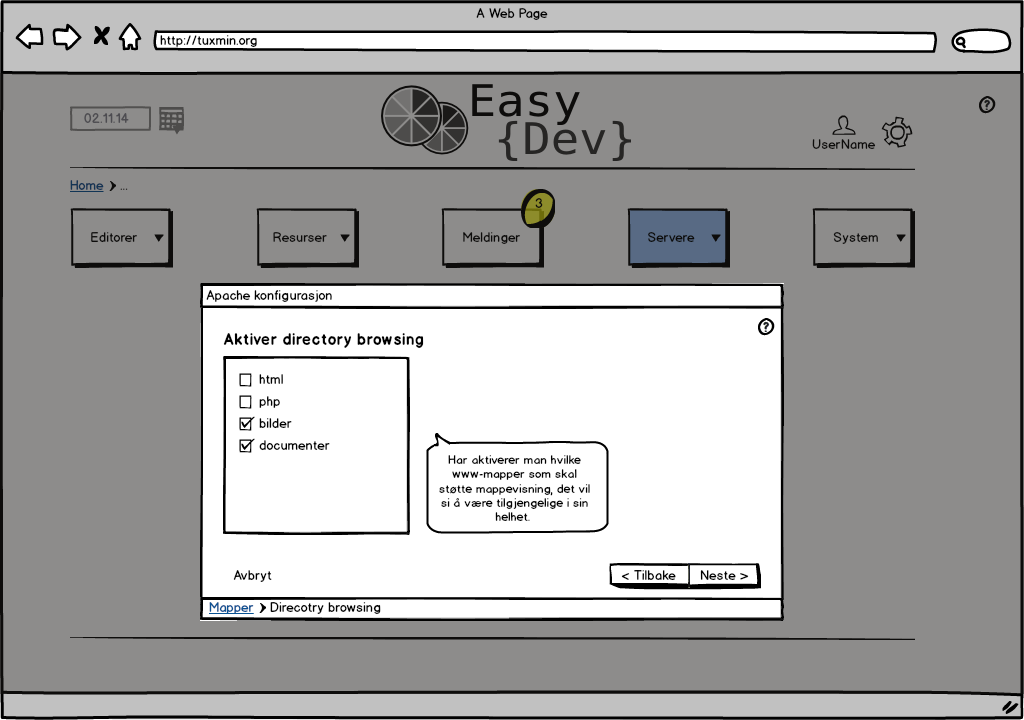
\includegraphics[width=\textwidth]
                {./img/prosessdokumentasjon/lowfi/apache3.png}
                \caption{Aktivere visning av innhold i mapper}
                \label{fig:apache3}
        \end{subfigure}
        \hspace{0.05cm}
        \begin{subfigure}[b]{0.48\textwidth}
                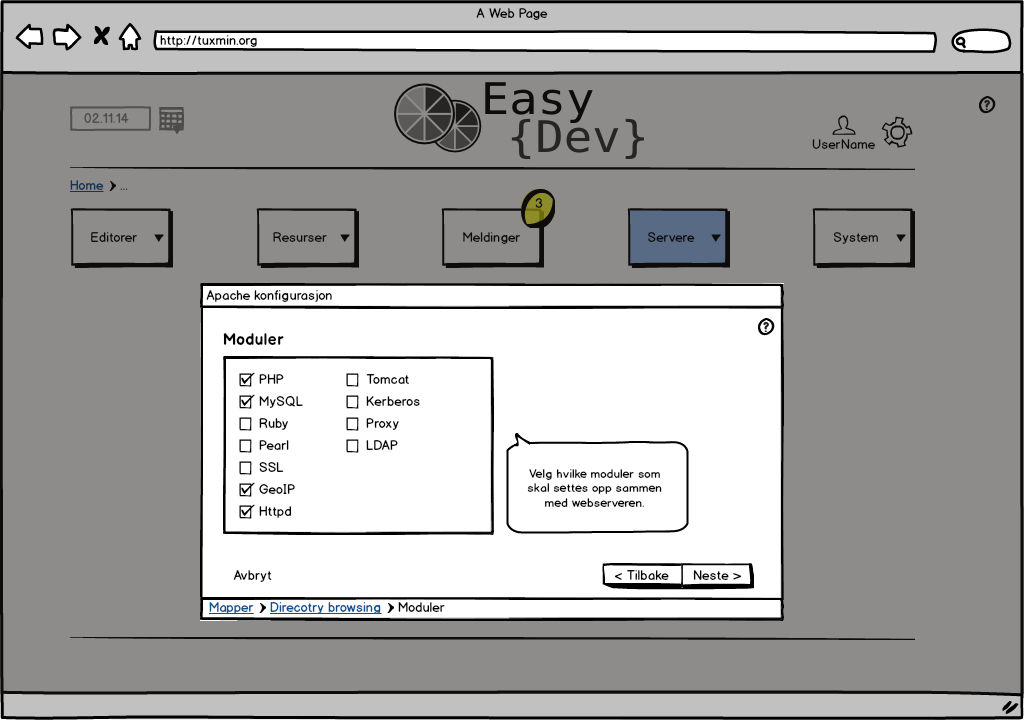
\includegraphics[width=\textwidth]
                {./img/prosessdokumentasjon/lowfi/apache4.png}
                \caption{Valg av moduler}
                \label{fig:apache4}
        \end{subfigure}
        
        \vspace{0.6cm}
        \begin{subfigure}[b]{0.48\textwidth}
                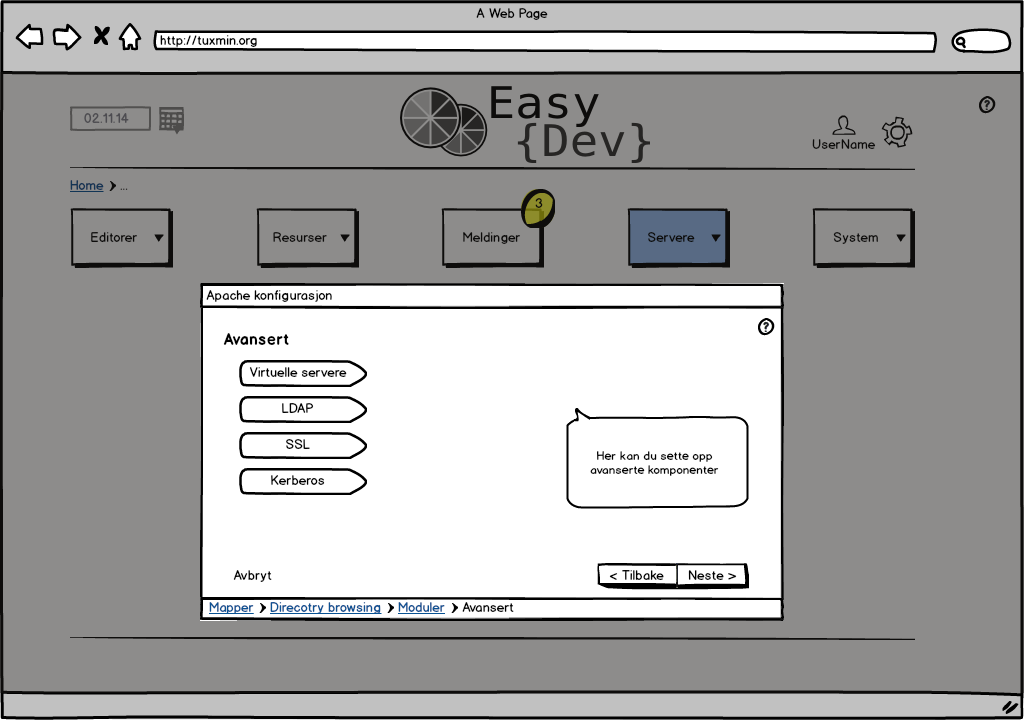
\includegraphics[width=\textwidth]
                {./img/prosessdokumentasjon/lowfi/apache5.png}
                \caption{Avanserte Apache moduler}
                \label{fig:apache5}
        \end{subfigure}
        \vspace{0.1cm}
        \caption[Konfigurasjon av Apache webserver]{Eksempel på konfigurasjon av Apache webserver.}\label{fig:lowfiapache}
\end{figure}


\subsection{Oppsett av brukere og grupper}
I følgende modul har vi mulighet til å sette både brukergrupper, brukere og rettigheter en enstake bruekre eller hele grupper av brukere. Modulen er tenkt å brukes da man tenker å benytte systemet for gruppearbeid slik at flere bruekere kan dele på samme resurser. De eksempler som beskrives her kan betraktes i figur \ref{fig:lowfibrukere}.

Vi begynner på samme måte som i forrige eksempel å starter på fremsiden (figur \ref{fig:brukere1}). Istedenfor å velge modul servere går vi til modul <<System>> som innholder flere undermoduler som kan brukes til oppsett og konfigurasjon av selve virtuelle maskinen og brukergrensesnittet. 
Vi kan derette (figur \ref{fig:brukere2}) sette opp en ny gruppe, slette gruppe eller gå videre med å legge til brukere til en gruppe. Under kontrollene ser vi også hvilke resurser som alerede er tildelt den gruppen og evntuelt kan vi fjerne disse rettigheter gjennom å sjekke en eller flere av alternativene.
Dersom vi ønsker å legge til nye bruekre i systemet vårt kan vi gjøre detet i neste skjermbilde (figur \ref{fig:brukere3}) og på en enkel måte gå videre og legge til eller slette brukere. 
% med flagg p setter vi hele denne figuren på en egen side
\begin{figure}
        \centering
        \begin{subfigure}[b]{0.48\textwidth}
                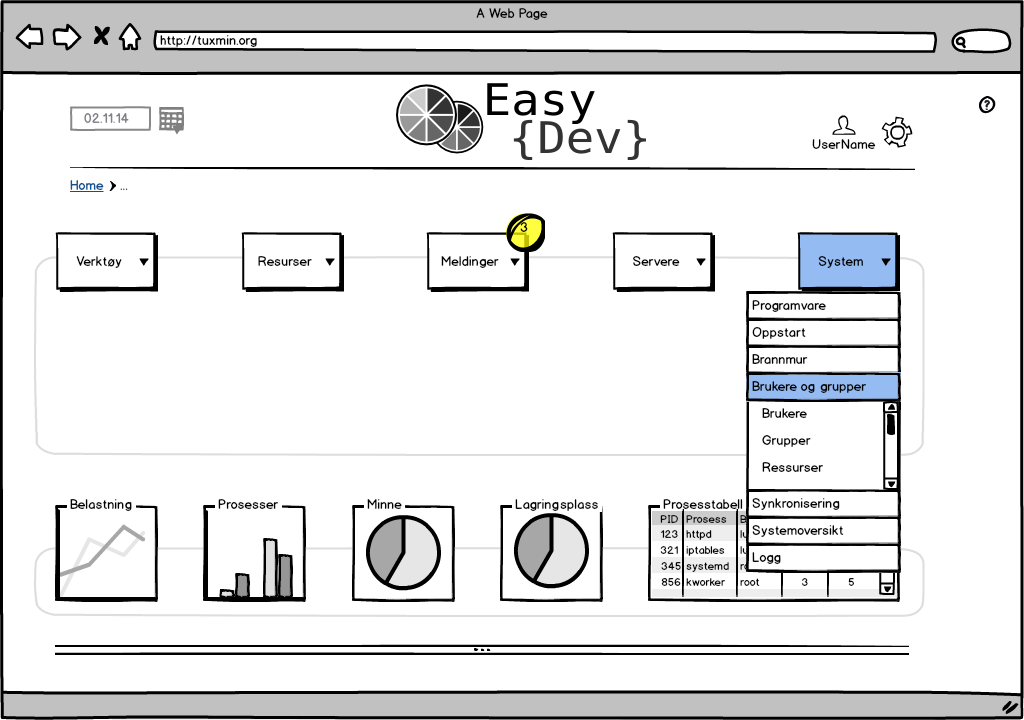
\includegraphics[width=\textwidth]
                {./img/prosessdokumentasjon/lowfi/b1.png}
                \caption{Fremside -> Velg brukeroppsett}
                \label{fig:brukere1}
        \end{subfigure}%
        ~ %add desired spacing between images, e. g. ~, \quad, \qquad, \hfill etc.
          %(or a blank line to force the subfigure onto a new line)
        \begin{subfigure}[b]{0.48\textwidth}
                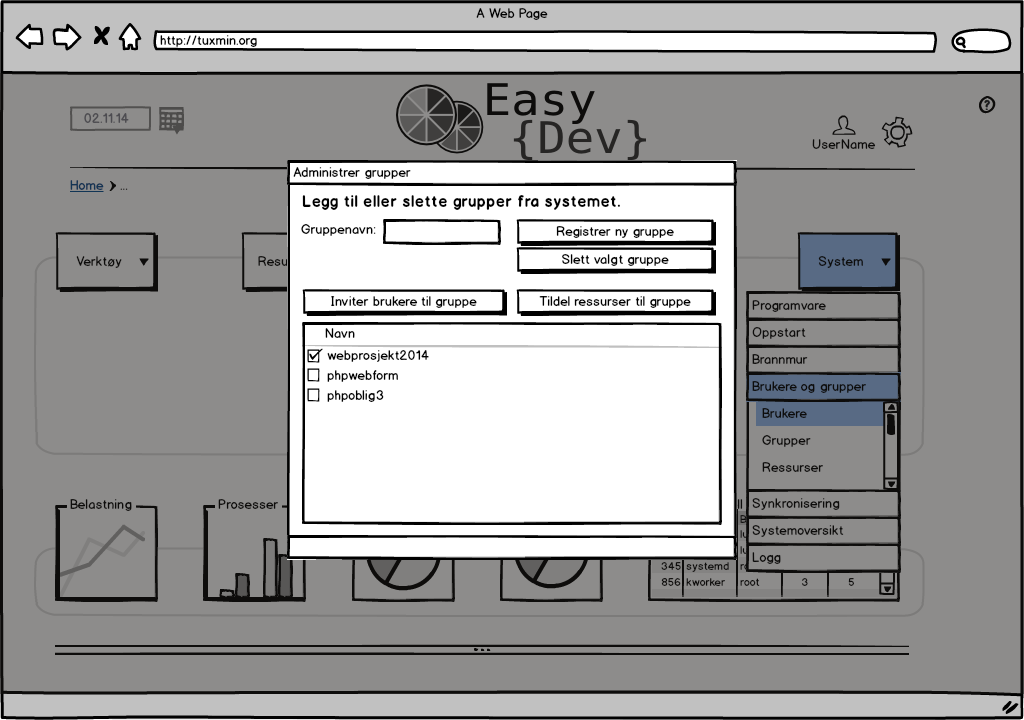
\includegraphics[width=\textwidth]
                {./img/prosessdokumentasjon/lowfi/b2.png}
                \caption{Grupper}
                \label{fig:brukere2}
        \end{subfigure}
       
        \vspace{0.6cm}
        \begin{subfigure}[b]{0.48\textwidth}
                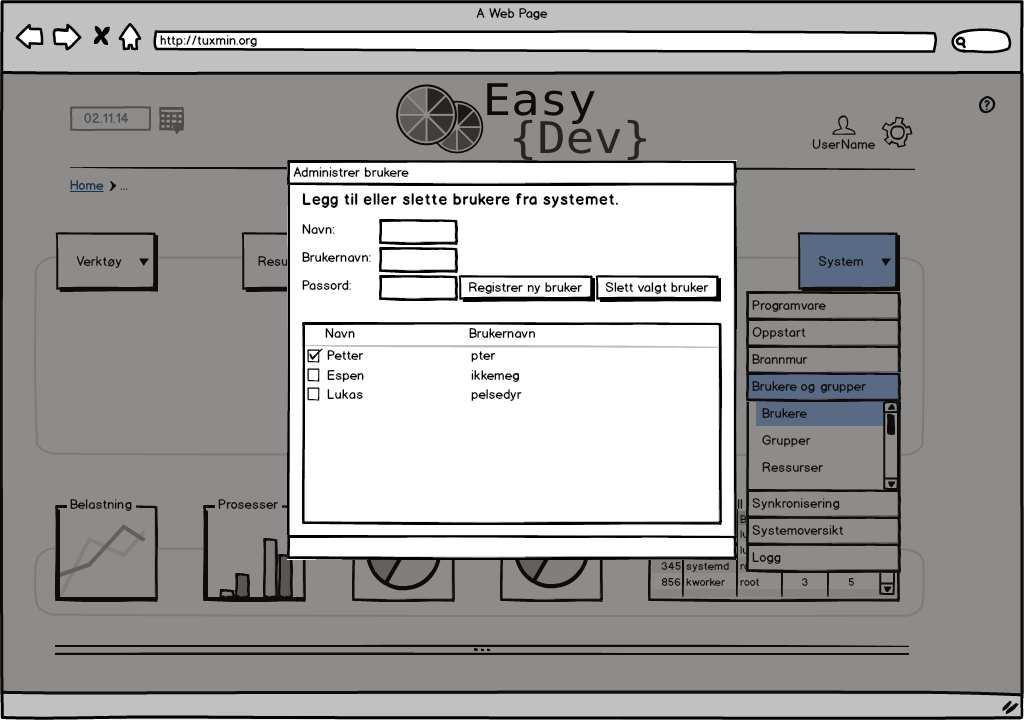
\includegraphics[width=\textwidth]
                {./img/prosessdokumentasjon/lowfi/b3.png}
                \caption{Brukere}
                \label{fig:brukere3}
        \end{subfigure}
        \hspace{0.02cm}
        \begin{subfigure}[b]{0.48\textwidth}
                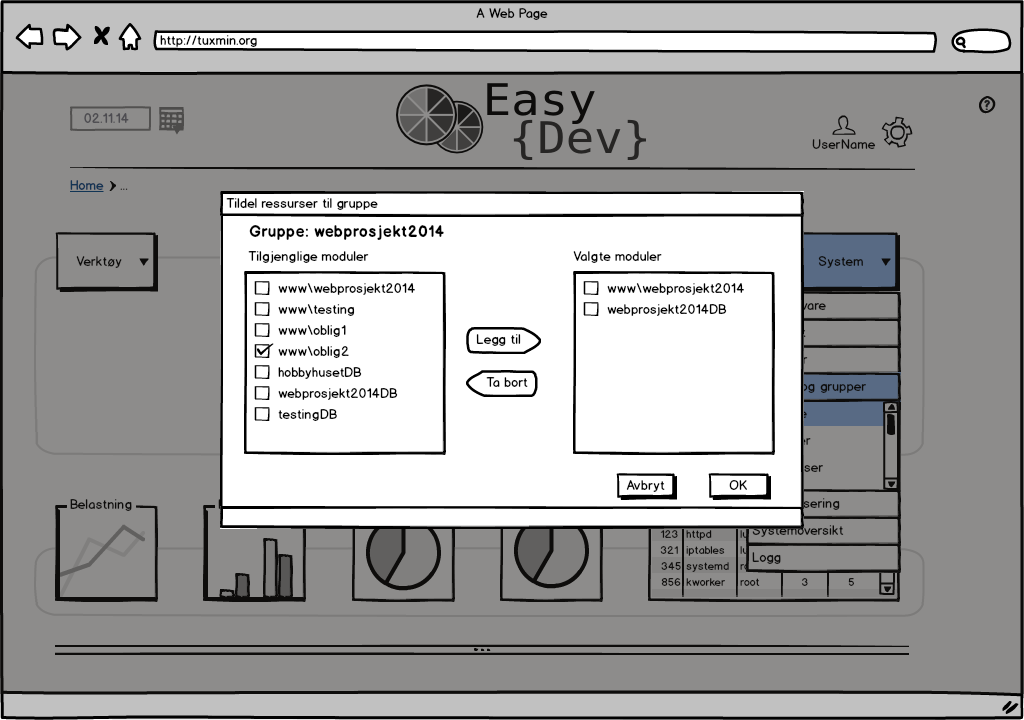
\includegraphics[width=\textwidth]
                {./img/prosessdokumentasjon/lowfi/b4.png}
                \caption{Moduler og resurser for gruppe}
                \label{fig:brukere4}
        \end{subfigure}
        \vspace{0.1cm}
        \caption[Konfigurasjon av brukere og grupper]{Eksempel på konfigurasjon av brukere og grupper.}\label{fig:lowfibrukere}
\end{figure}
Dersom vi ønsker kan vi gå videre til neste skjermbilde å legge til nye resurser som skal være tilgjengelige for spesifikk gruppe. Dette kan f.eks. dreie seg om en database, mappe alle sånn som tilgang til en konto på FTP server som kjører på systemet. 

\section{Hi-fi prototype}

\section{Kriterier og avgjøresler}
Fokuser på alle valg som ble tatt. Hvilke kriterier og 
prinsipper i faget ligger bak avgjørelsene? 

Her kan vi skrive om hvorfor vi har akkuratt valgt Linux. Hvorfor skal løsningen være webbasert og hvorfor skal den kjøres i en virtuell maskin? Og så andre kriterier og avgjøresel som vi har tatt under veien. 